\documentclass[12pt,aspectratio=169]{beamer}
\usetheme{metropolis}
\setbeamersize{text margin left=.5cm,text margin right=.5cm}
\usepackage[lf]{carlito}
\usepackage{siunitx}
\usepackage{tikz}
\usepackage{mathpazo}
\usepackage{bm}
\usepackage{mathtools}
\usepackage[ISO]{diffcoeff}
\diffdef{}{ op-symbol=\mathsf{d} }
\usepackage{xcolor,colortbl}


\setlength{\parskip}{0pt}
\renewcommand{\baselinestretch}{1}

\sisetup{
  inter-unit-product=\cdotp,
  per-mode=symbol
}
\tikzset{
  >=latex
}

\title{Topic 9: Fluid Mechanics}
\subtitle{AP and IBHL Physics}
\author[TML]{Dr.\ Timothy Leung}
\institute{Olympiads School}
\date{Updated: Summer 2022}

\newcommand{\pic}[2]{
  \includegraphics[width=#1\textwidth]{#2}
}
\newcommand{\eq}[2]{
  \vspace{#1}{\Large
    \begin{displaymath}
      #2
    \end{displaymath}
  }
}
%\newcommand{\iii}{\ensuremath\hat{\bm{\imath}}}
%\newcommand{\jjj}{\ensuremath\hat{\bm{\jmath}}}
%\newcommand{\kkk}{\ensuremath\hat{\bm{k}}}
%\newcommand{\iii}{\ensuremath\hat x}
%\newcommand{\jjj}{\ensuremath\hat y}
%\newcommand{\kkk}{\ensuremath\hat z}


\begin{document}

\begin{frame}
  \maketitle
\end{frame}



%\begin{frame}{Files for You to Download}
%  Please download the following files from the school website:
%  \begin{enumerate}
%  \item\texttt{PhysAP2-09-fluidMech.pdf}---The slides for this presentation. If
%    you want to print the slides on paper, I recommend printing 4 slides per
%    page.
%  \item\texttt{PhysAP2-10-thermodynamics.pdf}---The slides for the next topic.
%  %\item\texttt{15-16-Homework.pdf}---Homework assignment for Topics 15 and 16,
%  %  which cover Fluid Mechanics and Thermodynamics
%  \end{enumerate}
%  \vspace{.2in}Please download/print the PDF file before each class. When you
%  are taking notes, pay particular attention to details that aren't necessarily
%  on the slides.
%\end{frame}



\begin{frame}{Disclaimer}
  Fluid mechanics is part of the AP Physics 2 Exam, which does not require
  calculus. However, in the interest in completeness, \emph{some} calculus will
  be shown when deriving equations.
\end{frame}



\begin{frame}{What is a Fluid}
  \begin{itemize}
  \item The \emph{simple} (non-scientific) definition of a fliud is anything
    that \emph{flows}, which covers most gases and liquids
  \item\vspace{.1in}The \emph{scientific} definition of a fluid is \textbf{any
    substance that deforms \emph{continuously} under oblique stress}
    \begin{itemize}
    \item When a force (stress) is applied to a solid, it deforms until all the
      forces are balanced, and the deformation stops (e.g.\ stretching a spring)
    \item When a force is applied to a fluid, it continues to deform in shape as
      long as the force is present
    \item Fluid is continuous: it will fill all available space without gaps
    \end{itemize}
  \end{itemize}
\end{frame}



\begin{frame}{Density of a Fluid}
  The \textbf{density} $\rho$ of a fluid is defined as the mass of the fluid
  $m_\text{fluid}$ per unit volume $V_\text{fluid}$ that it occupies:
  
  \eq{-.2in}{
    \boxed{\rho=\frac{m_\text{fluid}}{V_\text{fluid}}}
  }
  \begin{itemize}
  \item Unit for density is \textbf{kilograms per meter cubed}
    (\si{\kilo\gram\per\metre\cubed})
  \item Below Mach number $M\approx 0.3$, density can be assumed to be constant
    throughout the fluid
  \item May be dependent on temperature by basic thermal expansion
  \end{itemize}
\end{frame}



\begin{frame}{Viscosity of a Fluid}
  \textbf{Viscosity} $\mu$ measures how ``thick'' a fluid is. It relates the
  rate of deformation ($\Delta u/\Delta y$) of the fluid to the shear stress
  $\tau$ that it experiences:

  \eq{-.2in}{
    \boxed{\tau = \mu\frac{\Delta u}{\Delta y}}
  }
  \begin{itemize}
  \item e.g.\ honey is more viscous than water.
  \item Shear stress is defined as $\tau=F/A$, with a unit of \textbf{pascal}
    (\si\pascal), which is the same as for pressure
  \item In AP Physics 2, we will mostly ignore viscous effects, as important as
    they are
  \end{itemize}
\end{frame}



\begin{frame}
  \frametitle{Hydrostatics}
  The fluid \textbf{pressure} on its density and depth:

  \eq{-.2in}{ \boxed{p=p_0+\rho_\text{fluid}gz} }
  
  where $g$ is the acceleration due to gravity, $z$ is the depth below the
  surface, and $p_0=\SI{1.01e5}\pascal$ is the atmospheric pressure at the
  surface.
  \begin{itemize}
  \item Pressure is the same in all directions
  \item Pressure is defined as force per unit area, and the unit is
    \textbf{pascal}:

    \eq{-.2in}{
      \boxed{p=\frac{F}A}\quad\quad\SI1\pascal=\SI1{\newton\per\metre\squared}
    }
  \end{itemize}
\end{frame}



\begin{frame}
  \frametitle{Pascal's Principle}
  If force is applied somewhere on a container holding fluid, the pressure
  increases \emph{everywhere} in the fluid, not just where the force is applied.

  \vspace{.3in} i.e.\ the pressure of the force will be transmitted into the
  fluid.
\end{frame}


\begin{frame}{Pressure with Different Fluids}
  \begin{columns}
    \column{.3\textwidth}
    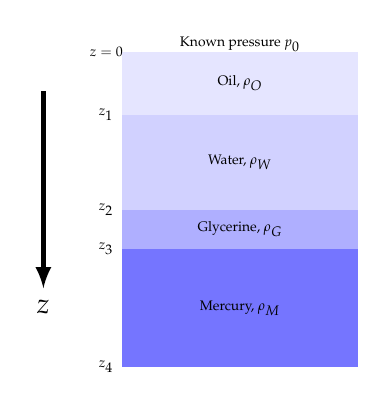
\begin{tikzpicture}
      \draw[ultra thick,->](-1,4.5)--(-1,2) node[pos=1,below]{$z$};

      %\fill[white!5!blue!80](0,0)   rectangle(3,1);
      \fill[white!10!blue!60](0,1)  rectangle(3,2.5);
      \fill[white!30!blue!45](0,2.5)rectangle(3,3);
      \fill[white!40!blue!30](0,3)  rectangle(3,4.2);
      \fill[white!50!blue!20](0,4.2)rectangle(3,5);
      \node at (-.2,5)  {\tiny $z=0$};
      \node at (-.2,4.2){\tiny $z_1$};
      \node at (-.2,3)  {\tiny $z_2$};
      \node at (-.2,2.5){\tiny $z_3$};
      \node at (-.2,1)  {\tiny $z_4$};
      %\node at (-.2,0)  {\footnotesize $z_6$};

      \node at (1.5,5.1) {\tiny Known pressure $p_0$};
      \node at (1.5,4.6) {\tiny Oil, $\rho_O$};
      \node at (1.5,3.6) {\tiny Water, $\rho_W$};
      \node at (1.5,2.75) {\tiny Glycerine, $\rho_G$};
      \node at (1.5,1.75) {\tiny Mercury, $\rho_M$};
    \end{tikzpicture}
    
    \column{.7\textwidth}
    For the fluid surface to remain \emph{static}, the fluid pressure on both
    side of the interface have to be equal. In this example:

    \vspace{-.45in}{\Large
      \begin{align*}
        p_1-p_0&=\rho_Ogz_1\\
        p_2-p_1&=\rho_Wg(z_2-z_1)\\
        p_3-p_2&=\rho_Gg(z_3-z_2)\\
        p_4-p_3&=\rho_Mg(z_4-z_3)\\\hline
        p_4-p_0&=\sum \Delta p
      \end{align*}
    }
  \end{columns}
\end{frame}



\begin{frame}{A Simple Example}
  \begin{columns}

    \column{.7\textwidth}
    \textbf{Example 1:} An aquarium is filled with water. The lateral wall of
    the aquarium is \SI{40}{\centi\metre} long and \SI{30}{\centi\metre} high.
    Using \SI{10}{\metre\per\second\squared} for the acceleration due to
    gravity, and \SI1{\gram\per\centi\metre\squared} for density of water, the
    force on the lateral wall of the aquarium is:
    \begin{enumerate}[(a)]
    \item\SI{36}\newton
    \item\SI{90}\newton
    \item\SI{180}\newton
    \item\SI{1500}\newton
    \end{enumerate}

    \column{.3\textwidth}
    \pic{1}{home-fish-tank}
  \end{columns}
\end{frame}



\begin{frame}{Example}
  \textbf{Example 2:} Consider the hydraulic jack in the diagram. A person
  stands on a piston that pushes down on a thin cylinder full of water. The
  cylinder is connected via pipes to a wide platform on top of which rests a
  1-ton (\SI{1000}{\kilo\gram}) car. The area of the platform under the car is
  \SI{25}{\metre\squared}; the person stands on a \SI{.3}{\metre\squared}
  piston. What is the lightest weight of a person who could successfully lift
  the car?
  \begin{center}
    \vspace{-.2in}
    \pic{.35}{jack}
    
    \vspace{-.2in}{\tiny Believe it or not, there \emph{is} someone who draws
      worse diagrams than Tim!}
  \end{center}
\end{frame}



\begin{frame}{A ``Manometer'' Example}
  \begin{columns}
    \column{.55\textwidth}
    \textbf{Example 3:} Pressure gauge $B$ is to measure the pressure at point
    $A$ in a water flow, as shown in the figure on the right. If the pressure at
    $B$ is \SI{87}{\kilo\pascal}, estimate the pressure at $A$, in
    \si{\kilo\pascal}. Assume all fluids are at \SI{20}\celsius. The densities
    of water, mercury and SAE 30 oil are, respectively:

    \vspace{-.3in}
    \begin{align*}
      \rho_\text{water}&=\SI{1000}{\kilo\gram\per\metre^3}\\
      \rho_\text{Hg}&=\SI{13600}{\kilo\gram\per\metre^3}\\
      \rho_\text{oil}&=\SI{890}{\kilo\gram\per\metre^3}
    \end{align*}
    
    \column{.45\textwidth}
    \pic{1}{mano}
  \end{columns}
\end{frame}



%\begin{frame}
%  \frametitle{Hydrostatic Example: Forces on a Hinge}
%  \begin{columns}
%
%    \column{.45\textwidth}
%    \begin{tikzpicture}
%      \begin{
%    \end{tikzpicture}
%    
%    \column{.55\textwidth}
%    The gate in the figure on the left is \SI{5}{m} wide, is hinged at point
%    $B$, and rests against a smooth wall at point $A$. Compute
%    \begin{enumerate}[(a)]
%    \item the force on the gate due to seawater pressure, and
%    \item the horizontal force $P$ exerted by the wall at point $A$, and
%    \item the reaction at the hinge $B$
%    \end{enumerate}
%  \end{columns}
%\end{frame}



\begin{frame}{Buoyancy: Everything Floats a Little}
  When an object is submerged inside a fluid
  \begin{itemize}
  \item The fluid exerts a pressure at the surface of the object
  \item By hydrostatics, the pressure is higher at the bottom than at the top
  \end{itemize}
  \begin{center}
    \pic{.3}{rock_fbvectors}
  \end{center}
\end{frame}



\begin{frame}{Buoyancy}
  Using some basic calculus (well, depends on who you ask), we can find the
  pressure over the entire surface to find the total buoyant force $\bm{B}$ the
  fluid exerts on the object. The expression is surprisingly simple:
  
  \eq{-.1in}{
    \boxed{\bm{B} = \rho_\text{fluid}gV\bm{\hat{k}}=
      m_\text{fluid}g\bm{\hat{k}}}
  }
  
  where $\rho_\text{fluid}$ is the density of the displaced fluid, and
  $V$ is the volume displaced. The direction of the force is upward. This
  equation is known as \textbf{Archimedes' principle}.
  
  \vspace{.25in}\textbf{Buoyant force has a magnitude that equals to the
    weight of the fluid displaced by the submerged object, pointing upward.}
\end{frame}



\begin{frame}{Buoyancy}

  \eq{0in}{
    \boxed{\bm{B} = \rho_\text{fluid}gV\bm{\hat{k}}=
      m_\text{fluid}g\bm{\hat{k}}}
  }

  Buoyancy does not depend on:
  \begin{itemize}
  \item the mass of the immersed object, or
  \item the density of the immersed object
  \end{itemize}

  \vspace{.15in}Objects immersed in a fluid have an ``apparent weight''
  $\bm{W}'$ that is reduced by the buoyant force:

  \eq{-.2in}{
    \bm{W}'=\bm{W}-\bm{B}=\rho'\bm{g}V
  }
  
  where $\rho'=\rho_\text{obj}-\rho_\text{fluid}$ is the relative density
\end{frame}



\begin{frame}{How Submarines Work}
  Like this:
  \begin{center}
    \pic{.7}{EbHMOXk}
  \end{center}
\end{frame}



\begin{frame}{How Submarines Work}
  Like all ships, a submarine does not naturally sink due to buoyancy. When a
  submarine submerges, water is pumped into the  ``ballast tanks'' in the hull
  hull to make the submarine heavier.
  \begin{center}
    \pic{1}{risinglemur}
  \end{center}
\end{frame}



\begin{frame}{Example}
  \begin{columns}
    \column{.7\textwidth}
    \textbf{Example 4:} An apple is held completely submerged just below the
    surface of a container of water. The apple is then moved to a deeper point
    in the water. Compared with the force needed to hold the water just below
    the surface, what is the force needed to hold it at a deeper point?
    \begin{enumerate}[(a)]
    \item Larger
    \item The same
    \item Smaller
    \item Impossible to determine
    \end{enumerate}

    \column{.3\textwidth}
    \pic{1}{apple.jpg}
  \end{columns}
\end{frame}



\begin{frame}{Example}
  \begin{columns}
    \column{.38\textwidth}
    \pic{1}{hpa_b}

    \column{.62\textwidth}
    \textbf{Example 5:} A salvage ship tries to raise a sunken miniature
    submarine from the bottom of Lake Superior. The submarine and its contents
    have a mass of \SI{72000}{\kilo\gram} and a volume of
    \SI{18.9}{\metre\cubed}.
    What upward force must be applied to raise the submarine? The density of
    water is \SI{1000}{\kilo\gram\per\metre\cubed}.
    \begin{enumerate}[(a)]
    \item\SI{1.8e5}\newton
    \item\SI{2.0e5}\newton
    \item\SI{4.8e5}\newton
    \item\SI{5.2e5}\newton
    \end{enumerate}
  \end{columns}
\end{frame}



\begin{frame}{Fluid Flow}
  \begin{center}
    As important as it is to understand hydrostatics,\\
    it's way more interesting when the fluid is moving!
  \end{center}
\end{frame}



\begin{frame}{Control Volume and Control Surfaces}
  A control volume ``CV'' is a fixed volume in which fluid is able to flow in
  and out of it. The surfaces of the control volume is called the control
  surface ``CS''.
  \begin{center}
    \pic{.5}{CV-CS}
  \end{center}
\end{frame}



\begin{frame}{Navier-Stokes Equations}
  The governing equations in fluid mechanics is called
  \textbf{Navier-Stokes equations}, which is written in complicated vector
  and calculus symbols:

  \vspace{-.35in}{\Large
    \begin{align*}
      \frac{\partial\rho}{\partial t} + \nabla\cdotp(\rho\bm{v})&=0\\
      \frac{\partial(\rho\bm{v})}{\partial t} +
      \nabla(\rho\bm{v}\otimes\bm{v}) &= -\nabla p +\bm{f}+\mu\nabla^2\bm{v}\\
      \frac{\partial e}{\partial t} + \nabla\cdotp(e\bm{v})&=
      -\nabla\cdotp p +\frac{1}{Re\; Pr}\nabla q +
      \frac{1}{Re}\nabla\cdotp(\tau\cdotp\bm{v})
    \end{align*}

  }
  Even for university students experienced with calculus, solving these
  equations is still a daunting task. \textbf{But what do they actually mean?}
\end{frame}

\begin{frame}{Continuity Equation}
  The first equation is called the \textbf{continuity equation}, which is the
  conservation of mass:

  \eq{-.2in}{
    \frac{\partial\rho}{\partial t} + \nabla\cdot(\rho\bm{v})=0
  }

  \textbf{Meaning:} The increase in fluid mass in a fixed volume containing a
  fluid is the amount of mass that flows in minus the volume that flows out of
  the volume.
\end{frame}


\begin{frame}{Momentum Equation}
  The second equation is the \textbf{momentum equation}, which is the 
  momentum-impulse theorem applied to fluids in a volume:

  \eq{-.15in}{
    \frac{\partial(\rho\bm{v})}{\partial t} +
    \nabla(\rho\bm{v}\otimes\bm{v}) = -\nabla p +\nabla\cdot\bm{\tau}
    +\rho\bm{g}
    %+\mu\nabla^2\bm{v}
  }

  \textbf{Meaning:} The increase in the total momentum of a fluid in a fixed
  volume is the sum of all the external forces (pressure, shear \& body forces)
  applied to the fluids, plus the change in momentum through the flow of
  particles in and out of the volume.
\end{frame}



\begin{frame}{Energy Equation}
  The third and final equation is the \textbf{energy equation}, which is the
  the work-kinetic energy theorem applied to fluids:
  
  \eq{-.2in}{
    \rho\frac{\partial e}{\partial t} + p(\nabla\cdotp\bm{v})=
    \nabla\cdotp(k\nabla T)+\Phi
  }

  \textbf{Meaning:} The increase in the internal energy of the fluid (i.e.\ the
  total kinetic energy of all the fluid particles) in a fixed volume is the
  work done by pressure forces, viscous forces (i.e.\ friction), plus the
  change in energy from the flow of fluid in and out of the volume.
\end{frame}



\begin{frame}{Let's Make Some Assumptions}
  For an ``ideal fluid flow'', we make the following assumptions to simplify
  the Navier-Stokes equation:
  \begin{enumerate}
  \item The flow is \textbf{steady}
    \begin{itemize}
    \item Flow is ``time independent'', i.e.\ does not change with time
    \end{itemize}
  \item The flow is \textbf{inviscid}
    \begin{itemize}
    \item The fluid has no viscosity
    \item No friction between the fluid and the surrounding, and therefore
    \item No shear stresses on the fluid
    \item Only forces are pressure at the surface, and body forces from gravity
  \end{itemize}
  \item The flow is \textbf{incompressible}
    \begin{itemize}
    \item Density is constant throughout
    \end{itemize}
  \end{enumerate}
\end{frame}



\begin{frame}{Assumptions for Ideal Fluid Flow}
  We will also assume that there is
  \begin{itemize}
  \item\textbf{no shaft work} done along the streamline
  \item\textbf{no heat transfer} along the streamline
  \end{itemize}
  Then the N-S equations reduces to the \textbf{Bernoulli equation}
  
  \eq{-.1in}{\boxed{
      p_1+\frac{1}{2}\rho v_1^2 + \rho gz_1=
      p_2+\frac{1}{2}\rho v_2^2 + \rho gz_2
    }
  }
  
  The term $\displaystyle\frac{1}{2}\rho v^2$ is called \textbf{dynamic
    pressure}, while $p+\rho gz$ is the \textbf{hydrostatic pressure}.
\end{frame}



%\begin{fame}
%  \frametitle{Flow Continuity}
%  Usually the continuity equation is written in \emph{differential form}, by
%  applying the \emph{divergence theorem} to the flux term:
%
%  \vspace{-.3in}{
%    \begin{align*}
%      \int_{CV}\frac{\partial\rho}{\partial t}dV+
%      \int_{CS}\rho\bm{v}\cdot d\bm{A}=&0\\
%    \end{align*}
%  }
%\end{frame}
%  \eq{-.15in}{
%    \boxed{\Phi_\text{V}=\int\bm{V}\cdot d\bm{A}}
%  }
%    
%  \vspace{-.1in}where $\bm{V}$ is the velocity (vector field) at the surface,
%  and $d\bm{A}$ is the infinitesimal area pointing \textbf{outwards}. We can
%  also expressed volume flux using the outward normal unit vector
%  $\hat{\bm{n}}$:
%
%  \eq{-.15in}{
%    \boxed{\Phi_\text{V}=\int\bm{V}\cdot\hat{\bm{n}}dA}
%  }
%\end{frame}
%
%\begin{frame}
%  \frametitle{Bernoulli Equation}
%
%  \eq{-.01in}{\boxed{
%      p_1+\frac{1}{2}\rho v_1^2 + \rho gz_1=
%      p_2+\frac{1}{2}\rho v_2^2 + \rho gz_2
%  }}
%\end{frame}
%
%
%\begin{frame}
%  \frametitle{Bernoulli Equation}
%
%  \eq{-.01in}{\boxed{
%      p_1+\frac{1}{2}\rho v_1^2 + \rho gz_1=
%      p_2+\frac{1}{2}\rho v_2^2 + \rho gz_2
%  }}
%
%  Bernoulli's equation is valid when
%  \begin{itemize}
%  \item the flow is \textbf{steady} (independent of time)
%  \item the flow is \textbf{incompressible}--compressibility (i.e. changes in
%    density of the fluid) effects are negligible for Mach number $M<0.30$
%  \item the flow \textbf{along a single streamline}
%  \item there is \textbf{no shaft work} done along the streamline between 1 and
%    2
%  \item there is \textbf{no heat transfer} along the streamline between 1 and 2
%  \end{itemize}
%\end{frame}



\begin{frame}{Bernoulli Equation}
  Regions where Bernoulli equation is valid:
  \begin{center}
    \pic{.8}{bernoulli}
  \end{center}
\end{frame}



\begin{frame}{Inlet Outlet Flow}
  \begin{center}
    \pic{.5}{physicsbook_fluids_graphik_26}
  \end{center}
  In this example, the mass flowing at the inlet is the same as the flow out of
  it:

  \eq{-.2in}{\boxed{\rho_1 v_1A_1=\rho_2 v_2A_2}}
  
  \vspace{-.15in}For constant fluid density, the $\rho$ terms on both sides of
  the equation will cancel:

  \eq{-.3in}{\boxed{v_1A_1=v_2A_2}}
\end{frame}



\begin{frame}{Example: Multiple Inlet \& Outlets}
  \begin{columns}

    \column{.43\textwidth}
    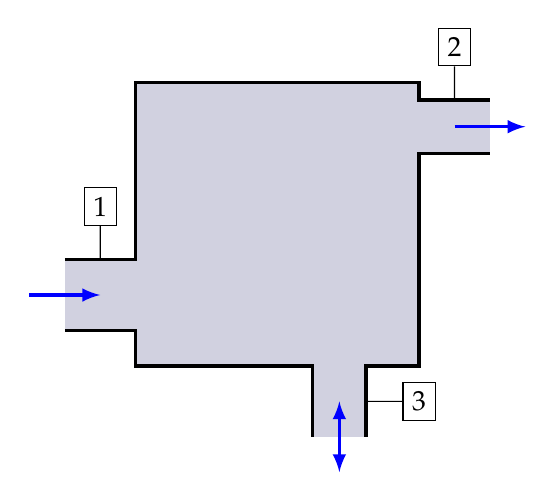
\begin{tikzpicture}[scale=.9]
      \fill[blue!20!gray!30](0,0) rectangle(4,4);
      \fill[blue!20!gray!30](2.5,0) rectangle(3.25,-1);
      \fill[blue!20!gray!30](-1,.5) rectangle(0,1.5);
      \fill[blue!20!gray!30](4,3) rectangle(5,3.75);
      \draw[very thick](-1,1.5)--(0,1.5)--(0,4)--(4,4)--(4,3.75)--(5,3.75);
      \draw[very thick](-1,0.5)--(0,0.5)--(0,0)--(2.5,0)--(2.5,-1);
      \draw[very thick](3.25,-1)--(3.25,0)--(4,0)--(4,3)--(5,3);
      \node[draw] at (-.5,2.25) (a) {1};
      \node[draw] at (4.5,4.5) (b) {2};
      \node[draw] at (4,-.5) (c) {3};
      \draw(-.5,1.5)--(a);
      \draw(4.5,3.75)--(b);
      \draw(3.25,-.5)--(c);
      \draw[->,very thick,blue](-1.5,1)--(-.5,1);
      \draw[->,very thick,blue](4.5,3.375)--(5.5,3.375);
      \draw[<->,very thick,blue](2.875,-.5)--(2.875,-1.5);
    \end{tikzpicture}

    \column{.57\textwidth}
    \textbf{Example 6:} Water at \SI{20}{\celsius} flows steadily through a
    closed tank, as shown in the figure. As section 1,
    $D_1=\SI{6}{\centi\metre}$ and the volume flow is
    \SI{100}{\metre\cubed\per\hour}. At section 2, $D_2=\SI{5}{\centi\metre}$
    and the average velocity is \SI{8}{\metre\per\second}. If
    $D_3=\SI{4}{\centi\metre}$, what is
    \begin{enumerate}
    \item the flow rate $Q_3$ in \si{\metre\cubed\per\hour}?
    \item the average $v_3$ in \si{\metre\per\second}?
    \end{enumerate}
  \end{columns}
\end{frame}



\begin{frame}{Example}
  \textbf{Example 7:} Find a relation between the nozzle discharge velocity
  $V$ and the tank free-surface height $h$. Assume frictionless flow.
  \begin{center}
    \pic{.35}{EGL}
  \end{center}

  \vspace{-.15in}{
    \footnotesize The line labelled ``EGL'' is called the
    ``energy grade line'', or the ``Bernoulli head'', given by the equation
    $h_0=z+p/\rho g+v^2/2g$. In the region where Bernoulli equation is valid,
    EGL is a constant.\par
  }
\end{frame}
\end{document}
